\documentclass[12pt,english]{article}
\usepackage{mathptmx}

\usepackage{setspace}

\usepackage{color}
\usepackage[dvipsnames]{xcolor}
\definecolor{darkblue}{RGB}{0.,0.,139.}

\usepackage[top=1in, bottom=1in, left=1in, right=1in]{geometry}
\usepackage{listings}
\usepackage{color}

%New colors defined below
\definecolor{codegreen}{rgb}{0,0.6,0}
\definecolor{codegray}{rgb}{0.5,0.5,0.5}
\definecolor{codepurple}{rgb}{0.58,0,0.82}
\definecolor{backcolour}{rgb}{0.95,0.95,0.92}

%Code listing style named "mystyle"
\lstdefinestyle{mystyle}{
  backgroundcolor=\color{backcolour},   commentstyle=\color{codegreen},
  keywordstyle=\color{magenta},
  numberstyle=\tiny\color{codegray},
  stringstyle=\color{codepurple},
  basicstyle=\footnotesize,
  breakatwhitespace=false,         
  breaklines=true,                 
  captionpos=b,                    
  keepspaces=true,                 
  numbers=left,                    
  numbersep=5pt,                  
  showspaces=false,                
  showstringspaces=false,
  showtabs=false,                  
  tabsize=2
}

%"mystyle" code listing set
\lstset{style=mystyle}
\usepackage{amsmath}
\usepackage{amstext}
\usepackage{amssymb}
\usepackage{setspace}
\usepackage{lipsum}

\usepackage{natbib}
\usepackage{url}
\usepackage{booktabs}
\usepackage[flushleft]{threeparttable}
\usepackage{graphicx}
\usepackage[english]{babel}
\usepackage{pdflscape}
\usepackage[unicode=true,pdfusetitle,
 bookmarks=true,bookmarksnumbered=false,bookmarksopen=false,
 breaklinks=true,pdfborder={0 0 0},backref=false,
 colorlinks,citecolor=black,filecolor=black,
 linkcolor=black,urlcolor=black]
 {hyperref}
\usepackage[all]{hypcap} % Links point to top of image, builds on hyperref
\usepackage{breakurl}    % Allows urls to wrap, including hyperref

\linespread{1.75}

\begin{document}

\begin{singlespace}
\title{Salary prediction of NBA Players based on 2016-2017 Season Performance using R \thanks{Thank you to Dr. Tyler Ransom, who has challenged and taught me more than I could imagine as it relates to coding and Data Science. Thank you to Mark Wissler, who's analytical thinking helped me organize my thoughts regarding this project and how to process the results. Thank you to Dr. Daniel Larson, who has been a mentor to me and my graduate liaison, who without, I would not be able to navigate the graduate program}}
\end{singlespace}
\author{Connor Cocklin \thanks{Department of Health and Exercise Science, Sports Data Analytics Lab, University of Oklahoma.\
E-mail~address:~\href{mailto:connorcocklin@ou.edu}{connorcocklin@ou.edu}}}

% \date{\today}
\date{May 9, 2019}

\maketitle


\begin{abstract}
 \begin{doublespace}
This project gathered performance data from the NBA 2016-2017 NBA season and used Linear Regression modelling to predict salary and identify undervalued players. Research questions include: What statistics have the greatest impact on predicted salary? What players are among the most underpaid according to the predictive model? Which of these players add the most value to their team by measure of Win Shares. The linear model used to predict salary included a variety of metrics and resulted in an $R^2 of .5.$ \\
\indent Culminating factors outside of performance explain the rest of the variance that the model did not. These include salary cap restrictions, years in the league, amount of all NBA appearances, Public Opinion, and free market factors and position demand at times of signings. A further investigation should look into how much revenue a player is predicted to bring an organization. This investigation would essentially look into the marginal revenue product of the NBA Player and would be free of the culminating factors outside of the relationship between salary and performance.
\end{doublespace}   
\end{abstract}

\vfill{}


\pagebreak{}


\section{Introduction}\label{sec:intro}
\linespread{2}
\begin{doublespace}
\indent This topic peaked my interest as a result of my curiosity into the financial workings of the NBA and other professional sports leagues.
There is a real need by sport organizations to be able to quantify both a players worth in value added by revenue brought to the organization and also 
a fair salary that fits within the predetermined and agreed salary cap restricting all teams within the league. NBA teams are not able to pay their players what
they bring in as fair as revenue because then there would be no marginal product (profit) generated to keep the organization wheel turning. When determining salary there
are many spokes with the wheel of the decision making process. Understanding how to quantify performance allows NBA organizations to build a team that maximizes wins 
while remaining under the salary cap restriction. The salary cap restriction for the 2016-2017 NBA season was set at $94.14 million$. With 12 active players this is an average of 
7.8 million per player. Performance by the players is not the only determinant when it comes to compensation as this will be showcased later when a performance based model is 
unable to completely explain variance within actual salary
paid to the players. Other work done by researchers have created other models which include factors outside of performance and in addition to performance measures to explain salary to 
a more successful model. This predictive model is the first portion of this project. \\
\indent In keeping with the theme of playing GM, this project will attempt to identify underpaid players among the NBA in the 2017 season and determine which of these players will maximize
wins when compared to their counterparts of the same position. The final result will be a team built to be as cheap as possible while maximizing wins. This project will showcase the analytical power of R as well as showcase the thought process of front offices within sport organizations in regards to deciding on team composition. There are many obstacles in choosing the right player for the best price for the organization and this will show a small glimpse into the issues that may arise when undertaking such an action. 
Unfortunately performance is not the end all be all for determining what a player should be paid when the general public might understand that to be the case, performance however is a major factor in that determination and in no way will hurt a player's justification for compensation. This data project hopes to build upon what many authors have contributed in the past and on data sets provided for public use through Kaggle by Omri GoldStein. This analysis was performed using RStudio desktop \cite{r13}. 

\end{doublespace}

\section{Literature Review}\label{sec:litreview}

\indent In the following section, we will take a look at 5 articles that add value to our interpretation of NBA player salary and the various factors that affect it. These articles will provide history of the models used to predict salary and the various avenues individuals have looked at to improving these models and then even expanding to the practicality of applying these different models in order to drive decisions and solve problems regarding free agency and talent evaluation.
\subsection{Wage and Nonwage Discrimination in Professional Basketball: Do Fans Affect It?}There have been a multitude of papers looking at performance and compensation for professional athlete's. Many other factors exist however, in \cite{10.2307/3487275} we see how fans and their racial bias's might play a role in compensation. The paper explores whether fans are a source of wage discrimination against African American players in the NBA. A multiple regression analysis found that black players are compensated fourteen to sixteen percent less than white players with comparable on-court performance. They also found that there exists statistically significant sorting by race based geographically but found that fan attendance does not move inversely of black players percentage of playing time. The authors of this study concluded that because white fans tend to want to see white players on the court there is an over representation of white player in large population areas composed of a relatively high proportion of white fans. This and the compensation of comparable black NBA players lead the authors to believe that there is a bias among the salary structure in the NBA. I believe this paper is important as it assesses factors outside of the players control. The players on court have the ability to control their performance. Ultimately in Utopian NBA performance would be the only factor deciding how to adequately compensate a player.
\subsection{Determinants of NBA Player Salaries.}
In the paper, \textit{Determinants of NBA Player Salaries} \cite{detersal132} the authors take a look at performance based measures to evaluate NBA Salary. The season data collected to be analyzed was from the 2013-2014 NBA season and included 243 NBA players. The authors hypothesized that scoring parameters such as points per game, field goal percentage, free throw, and three point percentage would be huge contributors towards determining salary. After they ran their analyses they found that not all their scoring measures were contributors to the extent they believed. Points per game, rebounds, and personal fouls were found to be among the stronger contributors towards determining NBA salary.
\subsection{Does One Simply Need to Score to Score?}
The paper title \textit{Does One Simply Need to Score to Score?} by \cite{BerriDavid2007DOSN} they begins with a literature review showcasing that players looking to maximize the amount of money they receive in a given contract should focus just on scoring points. He also offers an empirical investigation into why decision makers in the NBA seem to act inconsistently with a focus of winning games or maximizing profit for the club. There are some lessons that Berri points out through the paper that I will cover quickly. The first is that points scored overwhelmingly explain the evaluation of player productivity in the NBA. To give a more succinct explanation, a young Kyrie Irving depicting an old Uncle Drew explains, "This game has always been, and will always be, about buckets." The second, player productivity on the court creates wins, this means scoring points increases productivity the most which in turn results in "W's". The third is that team wins drive revenue. there have been two paradigms of thinking for a general manager of a sports team. There are win maximizing managers and revenue maximizing managers. Due to a large body of research on the matter, both styles seem to go hand in hand, and a win maximizing manager seems to reap all the benefits that a revenue maximizing manager would seek. The best summation of this review can be taken straight from the paper itself. "Players in the NBA need to \textbf{score} to score a major payday."
\subsection{Salary Determination in the Presence of Fixed Revenues}
In the paper \textit{Salary Determination in the Presence of Fixed Revenues} \cite{10095669220150201}, the authors look into determinants of compensation with fixed revenue. This paper gets behind economic principles behind marginal product and compensation. For firms to compete employees cannot pay them their marginal product or else there would be no money to cover overhead. That being said, this has been the case for firms when revenue is fixed. Since Berri is particularly inclined to study labor in sports, the authors and him have decided to take a look into salary determination in the NBA. The NBA has the majority of their revenue coming from Broadcasting rights which are agreed upon in wide time frames, essentially causing a majority percentage of their income to become "fixed". Berri et al. find that player salary in the NBA has become much more equalized and therefore changes in the player's bargaining power plays an important role in determining their salary. The bargaining position is tied particularly with performance on the court and popularity among fans. This popularity with fans helps players establish a better bargaining position. 
\subsection{Mixing the princes and the paupers: Pay and performance in the National Basketball Association}
In the paper \textit{Mixing the princes and the paupers: Pay and performance in the National Basketball Association} \cite{SIMMONS2011381} they had a primary research question revolving around disparity of pay in the NBA. The question was did players respond positively when disparity of salary among players in the team increased, or when there was a greater difference between higher and lower players did it have a negative or positive impact on team performance. They found that players responded positively generally or there was no negative effect. This is because of the "justified inequality", it is believed that players can concede that there are other players who are better than them and perform better. Thus, their performance on the court demands increased value in salary. Since this inequality of pay is justified by the value added of greater performance, players have no problem with disparity in salary among players on a team. The authors took a look at a "natural" experiment that occurred in the NBA in the 1996 season where the CBA raised salary caps and there was an extreme shift in disparity of salary. They found the players and teams responded positively which confirmed their suspicion of tournament theory. 

\vspace{3mm}
\indent
This body of research lays the basis of the initial part of my project where I recreate a regression fit for predicting salaries based on performance. The confounding factors introduced through some of these papers have inspired me to look toward finding the highest portion of Win Shares possible to access each players  worth and sort through players who are underpaid. 
\newpage
\section{Data}\label{sec:data}
The primary data set used was obtained through the public source Kaggle. Other sources of data were scraped from the  basketball reference web page. Data was cleaned in R and merged together in order to produce a master table and add flexibility.
\subsection{scraping, merging and cleaning the data}
Two data sets were downloaded from Kaggle as csvs and read into R:
\begin{singlespace}
\begin{lstlisting}
#reading in Data
seasonstats <- read.csv(file = "C:\\Users\\conno\\Desktop\\Data Science Class\\Final Project\\Seasons_Stats.csv", header = TRUE, sep = ",")

# Get salary dataset 
#Reading in salary dataset for year end 2017.
salary.table <- read.csv(file = "C:\\Users\\conno\\Desktop\\Data Science Class\\Final Project\\Salary1617.csv")

#cleaning data a tad, getting stats for year ending 2017.
stats17 <- 
  seasonstats %>% filter(Year >= 2017) %>% 
  select(Year:G, MP, PER, FG:PTS) %>% 
  distinct(Player, .keep_all = TRUE) %>% 
  mutate(MPG = MP/G, PPG = PTS/G, APG = AST/G, 
         RPG = TRB/G, TOPG = TOV/G, BPG = BLK/G, 
         SPG = STL/G,x3PaG = X3PA/G) 

#merging salary and stats into one table

Salary_Stats_2017 <- merge(stats17, salary.table,
                           by.x = "Player", by.y = "Player")
names(Salary_Stats_2017)[41] <- "Salary17"
Salary_Stats_2017<- Salary_Stats_2017[-39]
Salary_Stats_2017<- Salary_Stats_2017[-39]

#Reading in Advanced Statistics to join the party
#Get Advanced stats dataset
page <- read_html("https://www.basketball-reference.com/leagues/NBA_2017_advanced.html")
AdvancedStats.Table <- page %>% html_table(header = FALSE) %>% extract2(1)


#fixing headers and columns
names(AdvancedStats.Table) <- AdvancedStats.Table[1,]
AdvancedStats.Table <- AdvancedStats.Table[-1,]
AdvancedStats.Table <- AdvancedStats.Table[ , !names(AdvancedStats.Table) 
                                            %in% c("NA", "Tm", "PER", "MP", "Age")]

AdvancedStats.Table <- AdvancedStats.Table %>% filter(Rk!="Rk")


#changing column type to Numeric instead of Character
AdvancedStats.Table <- as.data.frame(AdvancedStats.Table)
AdvancedStats.Table <- as_tibble(AdvancedStats.Table)

AS1 <- AdvancedStats.Table %>% select(Rk, Player, Pos)
As2 <- AdvancedStats.Table %>% select(-Rk, -Player, -Pos)


As2 <- As2 %>% mutate_if(is.character,as.numeric)
AdvancedStats.Table <- bind_cols(AS1,As2)

AdvancedStats.Table = AdvancedStats.Table[!duplicated(AdvancedStats.Table$Player),]


#Merging data into Master data set

Master_Salary_Stats_2017 <- merge(Salary_Stats_2017, AdvancedStats.Table,
                           by.x = "Player", by.y = "Player")
\end{lstlisting}
\end{singlespace}

\subsection{}
In between the three separate data sources there existed data that was missing, incomplete, or corrupted. For the sake of filtering and ease, null data was omitted and the result left us with 310 observations or players to choose from. The Average salary was \$6,861,293 and the min and max were \$207,798 and \$30,963,450. The minimum salary for the NBA in the 2016-2017 season was \$543,471 per year but due to injuries or missed time lower salaries were dropped because they did not show enough of a sample size to merit tangible analysis. The salary low was set at \$200,000. Lebron James had the highest salary in the 2017 season. In the following section I will walk through the methods and procedure taken to ensure reproducible results.
\newpage

\section{Empirical Methods}\label{sec:methods}
I explored the data set presented to me with a multitude of combinations of standard and advanced metrics. I also looked for violations of multi-collinearity. Since my model is used to predict salary based on performance I did not need a high $R^{2}$. The key phrase here is based on performance, as seen in my literature review there are a multitude of variables that can be used to predict salary. As a result I have formed what I have deemed as the most appropriate model for my project which can be seen here:

\begin{equation}
\label{eq:1}
\resizebox{\textwidth}{!}{
Y_{p}=\beta_{i} + \beta_{1}MPG_{p} + \beta_{2}PPG_{p} + \beta_{3}APG_{p} + \beta_{4}RPG_{p} + \beta_{5}WS_{p} + \beta_{6}VORP{p} + \beta_{7}X3p._{p} + \beta_{8} AGE_{p}}
\end{equation}
where $Y_{p}$ is predicted salary for a given player $_p$, and $\beta$ are beta coefficients for a given player $_p$ performance measures used to predict salary.
\subsection{}
After this model allowed for the interpretation of underpaid and overpaid players in the 2016-2017 season we now must look towards finding the best team that maximizes win shares!\\
    Why win shares?\\
   \indent Win shares are my chosen proxy for assessing how much value an individual player brings to their team. \textbf{Win Shares} is a statistic that attempts to divvy up the credit for team success to the individuals on the team. It's calculated using player, team, and league-wide statistics. This statistic can be either positive or negative so you are able to see whether a player is helping or hurting their team due to the credit of wins or negative wins earned by them. In order to "play GM" we will need to follow the rules from the NBA in the 2016-2017 season and fill our roster appropriately without going over the salary cap. Other issues will be discussed further in the Findings and Conclusions. 
\newpage


\section{Research Findings}\label{sec:results}
The main summary table for the regression model can be found in Table \ref{Table1}. The Correlation matrix used for selecting appropriate measures can be found in Figure \ref{correlation}. An appropriate graphic showing a simple regression line plotted against salary and points per game can be found in Figure \ref{SalaryPPG}. This demonstrates the relational power performance statistics have on player compensation. 

\subsection{Team Builder}
\onehalfspacing
The salary cap for the 2016-2017 season was \$94.1 million. The salary cap floor was \$84.7 million. So I will have to spend at least to the floor while maximizing Win Shares. The league requires that teams carry a minimum of 13 players and that an average of 14 players per team. For the sake of this project we will have 13. There are 5 positions to be filled on the court at a time. We will include 2 players of each position and will fill the rest by greatest Win Shares.\\
Remember we have to reach a threshold of \$84.7 million. The chosen team can be seen here:
\begin{center}
\begin{tabular}{||c|c|c|c|c|c||}
\hline
 Player & Pos & WS & Salary & Running Total &\% Valued \\ [.5ex]
\hline
Rudy Gobert & C & 14.3 & \$2,121,288 & 2,121,288 &-\%161 \\ 
\hline
Nikola Jokic & C & 9.7 & \$1,358,500 & 3,479,788 &-\%121 \\
\hline
Gorgui Dieng & PF & 5.7 & \$2,348,783 & 5,828,571 & -\%104 \\
\hline
Blake Griffin & PF & 7.7 & \$20,140,839 & 25,969,410 & \%37 \\
\hline
Giannis Antetokounmpo & SF & 12.4 & \$2,995,421 & 28,964,831 & -\%101 \\
\hline
Jimmy Butler & SF & 13.8 & \$17,552,209 & 46,517,040 & \%22 \\
\hline
Lou Williams & SG & 6.1 & \$7,000,000 & 53,517,040 & -\%30.5 \\
\hline
Victor Oladipo & SG & 4.0 & \$6,552,961 & 60,070,001 & -\%24 \\
\hline
Isaiah Thomas & PG & 12.5 & \$6,587,132 & 66,657,133 & -\%94.6 \\
\hline
Stephen Curry & PG & 12.6 & \$12,112,359 & 78,769,492 & -\%02 \\
\hline
Myles Turner & C & 8.0 & \$2,463,840 & 81,233,332 & -\%75 \\
\hline
Gary Harris & SG & 4.6 & \$1,655,880 & 82,889,212 & -\%108 \\
\hline
T.J. Warren & SF & 4.1 & \$2,128,920 & \textbf{85,018,132} & -\%113 \\
\hline
\end{tabular}
\end{center}

\newpage
\doublespacing
This table displays each player selected to be apart of the team. While maximizing win shares I conceded some players who may have been considered "overpaid" in an effort to utilize their outstanding win share numbers. Through this analysis it is obvious that many of these players are on their rookie contract and playing at a super star level. Writing this in 2019 while looking back to the 2017 season we know many of these players who are paid low salaries have since been compensated fairly. Stephen Curry is now the highest paid player in the NBA at 37.46 million. Giannis is in the midst of leading the Bucks to a conference finals berth that hasn't happened since '01. \\
\indent The above column labeled "\% Valued" can be interpreted as percent over- or underpaid. So we see that in 2017 Rudy Gobert was paid a salary that underpaid his performance by \%161. We see that Blake Griffin was overpaid by \%37. Cumulative Win Shares are found to be 115.5. Now, if this team played every game in a season and went to the playoffs and played to game 7 every round there would only be 110 games. That being said Win Shares are meant to be interpreted in context of the team. So we would see decreased Win Shares on this team and we might even see negative win shares by players contributing less. 
\newpage

\section{Conclusion}\label{sec:conclusion}
In order to tie a nice bow on this project I would like to summarize my findings and expand on some steps moving forward.\\
\indent Moving forward I would have expanded up the model and created a dummy variably for those on rookie contract, also would've included years in the league. I would also expand by creating parallel models for underpaid players assessing importance of separate performance factors. For example, if everything remains equal what performance statistic drives predicted salary so far past actualized salary in underpaid players. Also, being able to adjust this model to filter out rookie contracts would be useful moving forward. An optimized model allowing to pick some arbitrary optimal trade off between difference in salary and win shares would be crucial moving forward. Also, getting the ability to switch out win shares for other proxies of value.\\
It is my hope that you enjoyed this exploration through the process of "playing GM" through analysis of the 2016-2017 season. 

\vfill
\pagebreak{}
\begin{spacing}{1.0}
\bibliographystyle{jpe}
\bibliography{Bibliography.bib}
\addcontentsline{toc}{section}{Bibliography}
\end{spacing}

\vfill
\pagebreak{}
\clearpage

%========================================
% FIGURES AND TABLES 
%========================================
\section*{Figures and Tables}\label{sec:figTables}
\addcontentsline{toc}{section}{Figures and Tables}
%----------------------------------------
% Figure 1
%----------------------------------------
\begin{figure}[ht]
\label{correlation}
\centering
\bigskip{}
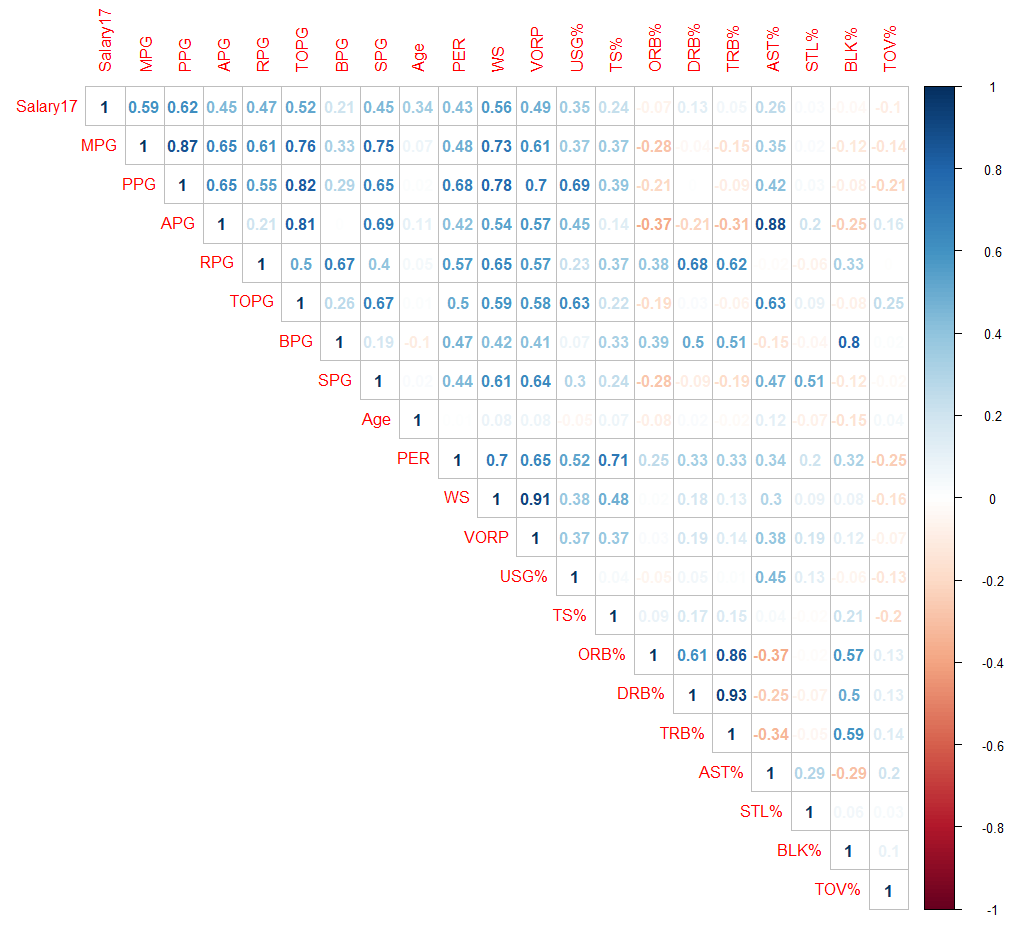
\includegraphics[width=.9\linewidth]{Pics/1.png}
\caption{Correlation matrix depicting various advanced and standard statistics and salary}
\label{fig:fig1}
\end{figure}

%----------------------------------------
% Figure 2
%----------------------------------------
\begin{figure}[ht]
\label{SalaryPPG}
\centering
\bigskip{}
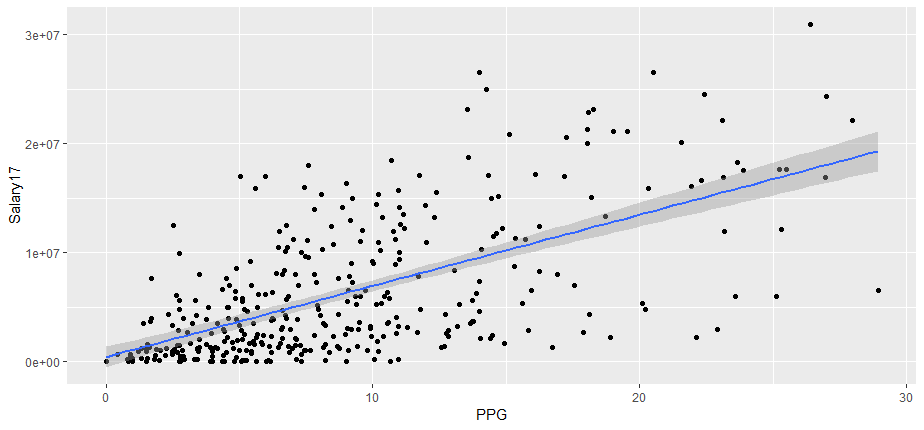
\includegraphics[width=.9\linewidth]{Pics/Salary17yPPGxPlot.png}
\caption{Simple Regression line with y = salary and x = points per game}

\end{figure}





%----------------------------------------
% Table 1
%----------------------------------------
\begin{table}[!htbp] \centering 
  \caption{Summary Table} 
  \label{Table1} 
\begin{tabular}{@{\extracolsep{5pt}}lc} 
\\[-1.8ex]\hline 
\hline \\[-1.8ex] 
 & \multicolumn{1}{c}{\textit{Dependent variable:}} \\ 
\cline{2-2} 
\\[-1.8ex] & log(Salary17) \\ 
\hline \\[-1.8ex] 
 MPG & 0.037$^{***}$ (0.013) \\ 
  PPG & 0.062$^{***}$ (0.018) \\ 
  APG & $-$0.016 (0.041) \\ 
  RPG & 0.048 (0.033) \\ 
  WS & 0.057 (0.050) \\ 
  VORP & $-$0.160$^{*}$ (0.092) \\ 
  X3P. & $-$0.341 (0.445) \\ 
  Age & 0.080$^{***}$ (0.011) \\ 
  Constant & 11.614$^{***}$ (0.337) \\ 
 \hline \\[-1.8ex] 
Observations & 310 \\ 
R$^{2}$ & 0.464 \\ 
Adjusted R$^{2}$ & 0.449 \\ 
Residual Std. Error & 0.830 (df = 301) \\ 
\hline 
\hline \\[-1.8ex] 
\textit{Note:}  & \multicolumn{1}{r}{$^{*}$p$<$0.1; $^{**}$p$<$0.05; $^{***}$p$<$0.01} \\ 
\end{tabular} 
\end{table} 

\newpage


%----------------------------------------
% Final Code
%----------------------------------------
\section{Code in R}
\begin{singlespace}
\begin{lstlisting}
library(tidyverse)
library(data.table)
library(GGally)
library(PerformanceAnalytics)
library(plotly)
library(rvest)
library(stringr)
library(magrittr)
library(corrplot)
library(vif)

#reading in Data
seasonstats <- read.csv(file = "C:\\Users\\conno\\Desktop\\Data Science Class\\Final Project\\Seasons_Stats.csv", header = TRUE, sep = ",")

# Get salary dataset 
#Reading in salary dataset for year end 2017.
salary.table <- read.csv(file = "C:\\Users\\conno\\Desktop\\Data Science Class\\Final Project\\Salary1617.csv")

#cleaning data a tad, getting stats for year ending 2018.
stats17 <- 
  seasonstats %>% filter(Year >= 2017) %>% 
  select(Year:G, MP, PER, FG:PTS) %>% 
  distinct(Player, .keep_all = TRUE) %>% 
  mutate(MPG = MP/G, PPG = PTS/G, APG = AST/G, 
         RPG = TRB/G, TOPG = TOV/G, BPG = BLK/G, 
         SPG = STL/G,x3PaG = X3PA/G) 

#merging salary and stats into one table

Salary_Stats_2017 <- merge(stats17, salary.table,
                           by.x = "Player", by.y = "Player")
names(Salary_Stats_2017)[41] <- "Salary17"
Salary_Stats_2017<- Salary_Stats_2017[-39]
Salary_Stats_2017<- Salary_Stats_2017[-39]

#Reading in Advanced Statistics to join the party
#Get Advanced stats dataset
page <- read_html("https://www.basketball-reference.com/leagues/NBA_2017_advanced.html")
AdvancedStats.Table <- page %>% html_table(header = FALSE) %>% extract2(1)


#fixing headers and columns
names(AdvancedStats.Table) <- AdvancedStats.Table[1,]
AdvancedStats.Table <- AdvancedStats.Table[-1,]
AdvancedStats.Table <- AdvancedStats.Table[ , !names(AdvancedStats.Table) 
                                            %in% c("NA", "Tm", "PER", "MP", "Age")]

AdvancedStats.Table <- AdvancedStats.Table %>% filter(Rk!="Rk")


#changing column type to Numeric instead of Character
AdvancedStats.Table <- as.data.frame(AdvancedStats.Table)
AdvancedStats.Table <- as_tibble(AdvancedStats.Table)

AS1 <- AdvancedStats.Table %>% select(Rk, Player, Pos)
As2 <- AdvancedStats.Table %>% select(-Rk, -Player, -Pos)

As2 <- As2 %>% mutate_if(is.character,as.numeric)
AdvancedStats.Table <- bind_cols(AS1,As2)

AdvancedStats.Table = AdvancedStats.Table[!duplicated(AdvancedStats.Table$Player),]

#Merging data into Master data set

Master_Salary_Stats_2017 <- merge(Salary_Stats_2017, AdvancedStats.Table,
                           by.x = "Player", by.y = "Player")
#correlation 
library(corrplot)
correlations <- cor(Master_Salary_Stats_2017%>%
                      select(Salary17, MPG:SPG,
                             Age, PER, x3PaG,eFG.,contains("%")),
                    use = "complete.obs", method = "pearson")
corrplot(correlations, method = "number", type = "upper")
       
#Correlation hierarchy to Salary is PPG>MPG>TOPG>RPG=PER>APG=SPG>BPG>X3P>eFG
#The above is the first set of variables, because of level of correlation of X3pag and eFG I decided to read in more advanced statistics.
#These measures include value over replacement player and usage rate
correlations1 <- cor(Master_Salary_Stats_2017 %>%
                      select(Salary17, MPG:SPG,
                             Age, PER, WS, VORP,`USG%`,contains("%")),
                    use = "complete.obs", method = "pearson")
corrplot(correlations1, method = "number", type = "upper")
#We see that the advanced stats add some explaination to the bigger picture of what drives salary.
#Here TOV% corrects for where TOPG seemed to moderately positively correlate with pay while widly being considered a negative play
#If we take all factors of with correlation higher than .3 we have a hierarchy that looks like:
# PPG>MPG>WS>VORP>RPG>APG>SPG>PER>USG%>AGE
#Scatter Plot with regression line
Master_Salary_Stats_2017 %>%
  ggplot(aes(x = PPG, y = Salary17)) + 
           geom_point() +
           geom_smooth(method = "lm")

Master_Salary_Stats_2017 %>%
  ggplot(aes(x = MPG, y = Salary17)) +
    geom_point() +
  geom_smooth(method = "lm")

Master_Salary_Stats_2017 %>%
  ggplot(aes(x = VORP, y = Salary17)) +
  geom_point() +
  geom_smooth(method = "lm")

#Regression Analysis
#Regression based on per game stats
SAL_lmGM = Master_Salary_Stats_2017 %>%
  select(Salary17, MPG:SPG)
PERGAME_MODEL <- lm(log(Salary17) ~., data = SAL_lmGM)
summary(PERGAME_MODEL)

#Kicthen Sink significant at MP, FG, FGA, ORB, DRB, AST, MPG, PPG, APG, RPG,
#AST%, TOV%, will move to create best fit model

SAL_BEST = Master_Salary_Stats_2017 %>%
  select(Salary17, MP, FG, FGA, ORB, DRB, AST, MPG, PPG, APG, RPG, `AST%`,`TOV%`)
LM_BestFIT <- lm(Salary17~., data = SAL_BEST)
summary(LM_BestFIT)
#DIDNOT PRODUCE 
#WILL NOW GUESS WHICH STATS PRODUCE BEST MODEL
SAL_GUESS = PractiveDropLowSalaries %>%
  select(Salary17, MPG, PPG, APG, RPG, WS, VORP, X3P., Age)
LM_GUESS <- lm(log(Salary17)~., data = SAL_GUESS)
summary(LM_GUESS)

car::vif(LM_GUESS)
#accessing residuals and createing seperate df
#removing NAs in data
PracticeNAremove <- Master_Salary_Stats_2017
PracticeNAremove <- PracticeNAremove %>% drop_na("MPG","PPG", "APG", "RPG", "WS", "VORP", "X3P.","Age")

PractiveDropLowSalaries <- PracticeNAremove[!(PracticeNAremove$Salary17 <=200000),]

Practice <- PractiveDropLowSalaries %>% select(Player, Pos.y, Salary17, WS)
Practice$LogSalary17 <- log(Practice$Salary17)

Practice$DifferenceSalary17 <- residuals(LM_GUESS)
Practice <- Practice %>% select(-PredictedSalary17)
Results <- Practice

summary(LM_GUESS)
library(stargazer)
stargazer(LM_GUESS, type = "latex", out = "LM_Guess.txt",
          no.space = TRUE, single.row = TRUE, title = "Summary Table", omit.stat = "f","ll","ser")


\end{lstlisting}
\end{singlespace}

\end{document}